\section{Visualization Infrastructure}
In this section, we present certain key aspects of our web-based visualization
infrastructure. This infrastructure facilitates the integration of arbitrary
views to Parceive by providing a common interface for accessing abstracted
runtime traces. The biggest challenge when dealing with traces is the
potentially overwhelming amount of data. Often this leads to unmanageable views
with unpractical delays. Our visualization infrastructure addresses this
problem by building upon a highly reactive client-server architecture (see
Figure \ref{fig:visualization}) that provides four key services: (a) trace
optimization, (b) on-demand loading, (c) caching and pipelining, and (d)
state management and communication.

\begin{figure}[h!]
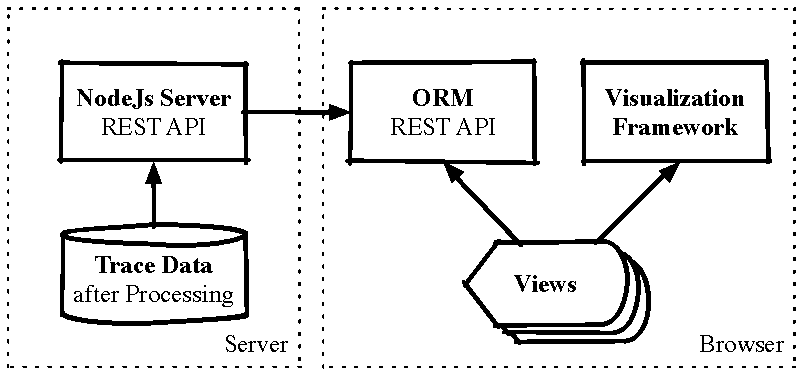
\includegraphics[width=\linewidth]{img/visualization_framework}
\caption{The visualization infrastructure of Parceive.}
\label{fig:visualization}
\end{figure}

\paragraph{Trace Optimization}
Parceive uses file-based databases to store trace data. Its layout is tuned for
write operations to reduce the runtime overhead. All the information required
by the views can be obtained by performing database queries. However, most of
the read operations would take a disproportionate amount of time to complete
without applying certain optimizations on the trace database. Hence, we perform
a set of optimizations during a post-processing step to reduce lookup times for
views

The most important optimization is the insertion of table indexes for enabling
highly efficient search strategies by the database. Another optimization is the
creation of intermediary tables to avoid expensive joins for most queries.
Since this operation adds no additional trace data, creating redundancy
generates no overhead and does not increase the overall complexity. Another
optimization is the reduction of fragmentation within data tables. As
result, the increased data locality speeds up queries and has a considerable
effect on ones that require a full table scan. Additionally, the fragmentation
considerably reduces the size of the trace databases.

\paragraph{On-Demand Loading}
On-demand loading of trace data is a service that improves the responsiveness
of the visualization. Often, loading entire traces into the browser is not
possible due to memory restrictions. To solve this problem, a NodeJS server was
developed that reads data on demand. The server exposes a REST \cite{rest} API
to manage the retrieval of data. For security reasons, all SQL queries are
contained in this server without supporting arbitrary queries. The
implementation makes use of multiple parallel reads to the same database to
reduce the latency and throughput when large amounts of data are requested by
the views. This service let users seamlessly navigate and explore software
systems that produce a potentially unmanageable amount of trace data.

\paragraph{Caching and Pipelining}
On the client side, we provide a Object Relational Mapper (ORM) module to
simplify development and improve responsiveness by using caching. This module
enables accesses to predefined entities and navigate the relationships between
them. The corresponding API is implemented using promises \cite{promises}
simplifying the asynchronous and parallel behavior. The greatest benefit for
views using this ORM are the provided optimizations to the data loading scheme.
The most important ones are caching and pipelining. Caching allows the ORM to
avoid loading data that has been accessed before. Pipelining combines multiple
queries to the same endpoint into a single one. When requesting a large number
of entities, pipelining heavily improves the throughput with only small
latency overhead.

\paragraph{State Management and Communication}
The visualization framework provides global state management and communication
facilities to views. The former is based on a centralized and persistent state
storage that allows to retain the state of views across page loads. Currently,
the view layout and the marked nodes are automatically stored as part of the
state. In addition, each view can save tailored information at any time and
retrieve it during rendering. Local storage is used to house all the state
information making it persistent. This service reduces computational effort for
views by reusing results across arbitrary UI events.

The communication service empowers arbitrary views to interact by triggering
predefined events. These events let users explore their traced applications
with a combination of synchronized representations on complementary viewpoints.
One example is the simultaneous highlighting of entities on different views to
improve the ease of use. Another example is the spotting of distinct entities
for further inspection on separate views. This use-case may alleviate the
scalability problem of views by reducing the amount of nodes to be displayed.
Currently there are three types of communication provided:

\begin{itemize}
	\item \textit{Focusing} brings entities to the attention of the user by
centering the respective representations on all views.
	\item \textit{Marking} allows to communicate selected entities between views.
	\item \textit{Spotting} replaces the shown entities in views by a new
collection of entities.
	\item \textit{Hovering} highlights entities on multiple views by reducing the
opacity of all other entities.
\end{itemize}